\documentclass[10pt]{article}

\usepackage{amssymb,amsfonts,amsmath,amsthm}
\usepackage{algorithm,algpseudocode}
\usepackage{enumitem}
\usepackage{graphicx}
\usepackage{mathtools}
\usepackage{multicol,fullpage}
\usepackage{url}
\usepackage{subfigure}
\usepackage{xltxtra,fontspec,xunicode}
\defaultfontfeatures{Scale=MatchLowercase}
\setmonofont{VTScreenplayUnderwoodB}

\DeclarePairedDelimiter\abs{\lvert}{\rvert}
\DeclarePairedDelimiter\norm{\lVert}{\rVert}
\DeclarePairedDelimiter\parens{(}{)}
\DeclarePairedDelimiter\curly{\{}{\}}
\DeclarePairedDelimiter\ceil{\lceil}{\rceil}
\DeclarePairedDelimiter\floor{\lfloor}{\rfloor}

%% star versus non-star.
\makeatletter
 \let\oldabs\abs
 \def\abs{\@ifstar{\oldabs}{\oldabs*}}
 \let\oldnorm\norm
 \def\norm{\@ifstar{\oldnorm}{\oldnorm*}}
 \let\oldparens\parens
 \def\parens{\@ifstar{\oldparens}{\oldparens*}}
\makeatother

\algnewcommand{\LineComment}[1]{\State \(\triangleright\) #1}

\newcommand{\suchthat}{\, \mid \,}
\newcommand{\bigO}[1]{\mathcal{O}{\parens{#1}}}
\newcommand{\bigOmega}[1]{\Omega{\parens{#1}}}
\newcommand{\bigTheta}[1]{\Theta{\parens{#1}}}
\newcommand{\littleO}[1]{o{\parens{#1}}}
\newcommand{\littleOmega}[1]{\omega{\parens{#1}}}

\newcommand{\kmax}{k_{\max}}
\newcommand{\logkmax}{\log_{2}{\kmax}}
\newcommand{\topk}[2]{\mathrm{top}_{#1}\parens{#2}}
\newcommand{\topkmax}[1]{\topk{\kmax}{#1}}
\newcommand{\dataset}{\curly{f_{i}}}
\newcommand{\bigassexpression}{\bigO{ \frac{N}{B}\alpha \parens{\frac{N}{B}} \parens{\sqrt{\log{\frac{N}{B}}} + \log{\frac{\kmax}{B}}}} }

\newcommand{\listj}{\texttt{list}_{j}}
\newcommand{\tmplist}{\texttt{list}}
\newcommand{\tmptopk}{\texttt{topk}}
\newcommand{\tree}{\texttt{tree}_{j}}
\newcommand{\key}{\texttt{key}}
\newcommand{\val}{\texttt{value}}

\newcommand{\na}{\textit{n/a}}
\newcommand{\ditto}{\textit{do.}}


\newtheorem{lemma}{Lemma}

\hyphenation{Geo-Wave}
\hyphenation{Geo-Mesa}
\hyphenation{Geo-Trellis}
\hyphenation{Simple-Feature}
\hyphenation{Simple-Feature-Type}

\begin{document}

\title{GeoMesa and GeoWave Comparative Analysis: Final Report}

\author{Azavea, Inc.}

\date{}

\maketitle

\begin{abstract}
  This document details the results of a comparative analysis between two open source geospatial big data frameworks: GeoWave and GeoMesa.
  A feature comparison and a set of performance tests with analysis are presented.
  We have concluded that despite a large set of overlapping features, specifically the capability to index and query spatial and spatiotemporal data in Accumulo, the projects differ from each other in substantial ways.
  Through analyzing performance test data, we make four conclusions about the performance characteristics of the current versions of the systems - GeoMesa 1.2.6 and GeoWave 0.9.3 - for the use case of indexing spatial and spatiotemporal data in Accumulo: (1) GeoMesa performed better against queries with large result counts - i.e. queries that were not highly selective - while GeoWave performed better on smaller result sets - i.e. queries that selected fewer results out of a larger dataset; (2) GeoWave performed better against queries with larger temporal bounds, while GeoMesa performed better when the temporal bounds were smaller (around a couple of weeks or less); (3) GeoMesa performed better in the non-point dataset use case; and (4) GeoWave outperformed GeoMesa in multitenancy use cases, where there are 16 to 32 queries being executed against the system in parallel.
  We also find the two systems perform reasonably well in all cases, and that neither system was dominant in performance characteristics.
  We conclude by providing recommendations for ways the two projects can collaborate moving forward in light of this analysis.
\end{abstract}

\begin{multicols}{2}
  \section{Introduction}
\label{sec:introduction}

GeoMesa and GeoWave are two open source projects that deal with large geospatial data.
At a high level, these projects offer solutions to many of the same types of problems.
Because of this overlap, it has been difficult for new users approaching the big geospatial data community to understand what the differences are between these projects and what project should be used under what circumstances.
For some of their most overlapping functionality, for example, indexing spatial and spatiotemporal data in Accumulo, the differences between the two projects can be unclear even to veterans of big geospatial data processing.
This document aims to address this lack of clarity by discussing the many significant differences between the projects;
differences in form, function, and performance.

In the summer of 2016, Azavea conducted a comparative analysis of GeoWave and GeoMesa in order to gain a deeper understanding of the two projects and to share that understanding with the geospatial big data community.
This document contains the results of our efforts and aims to provide a more clear picture of how the projects are different from each other and what use cases fit best to either project.
We hope this will aid the geospatial big data community in gaining a deeper understanding of these two outstanding projects and allow a better utilization of their functionality.

Along with an understanding how the projects are different from each other, this comparative analysis aims to provide information and guidance to potential future collaboration efforts between the GeoWave and GeoMesa projects.

This document assumes prior knowledge about the GeoMesa and GeoWave projects and is not intended to be an introduction to those projects.
For background information, please see the project websites:


\begin{itemize}
\item  GeoWave: \url{http://ngageoint.github.io/geowave/}
\item  GeoMesa: \url{http://www.geomesa.org/}
\end{itemize}

  \section{Feature Comparison}
\label{sec:featurecompare}

The GeoMesa and GeoWave projects contain many features that overlap, and many that do not.
The Venn diagram shown in Figure \ref{venn} is not a complete list of features,
but indicates the significant overlap of the core features of GeoWave and GeoMesa and some of the distinguishing features that set them apart.

\begin{figure}[h!tb]
  \centering
  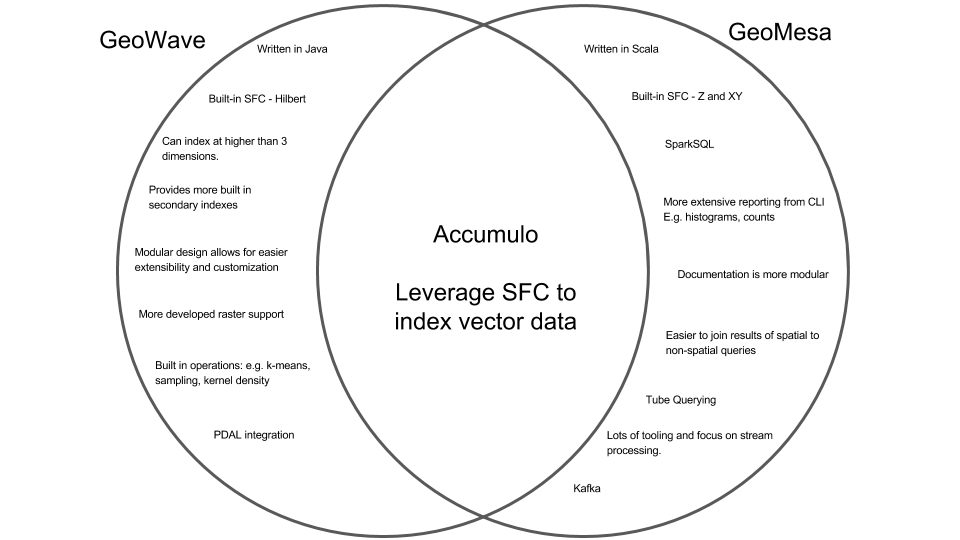
\includegraphics[width=0.60\textwidth]{../docs/img/venn-diagram.png}
  \caption{Venn Diagram of features.}
  \label{venn}
\end{figure}

As is illustrated in the diagram, there is a major overlap when it comes to a core feature of the two projects, namely using space filling curves to index geospatial data in Accumulo.
However, there are many features that differentiate the projects from one another.
Below is a summary table of feature similarities and differences.
A more detailed list of features can be found in Appendix \ref{appendix:features}: Details of GeoMesa and GeoWave features.

\subsection{Generality of the Architecture}
\label{sec:featurecompare:generality}

A major difference between the projects is the generality of the architectures when it comes to supporting
various backends\footnote{Backend refers to the specific mechanism for storing vector, data and the related geospatial index (ex: Accumulo, HBase).}
and indexing strategies.
GeoWave API has a focus on being an N-Dimensional indexing mechanism for arbitrary backends.
The fact that this document focuses on its ability to handle geospatial data ($2$-Dimensional spatial and $3$-Dimensional spatiotemporal data) is only based on the currently known GeoWave use cases.
However, the project aims at supporting data with arbitrary dimensionality.
GeoMesa API, on other hand, is directly tailored to geospatial indexing allowing for clearer interface, implementation, and paths for optimization.

GeoWave specifically is designed around abstractions that remain agnostic about the storage and access implementations.
This could provide more flexibility for developing backend support, which might explain why GeoWave HBase support is more mature than GeoMesa's.
GeoMesa focuses on using GeoTools' abstractions, and thus is more dependent on GeoTools as a base library.
GeoMesa also focuses less on dealing with abstractions; this may have an effect that features written for one backend are difficult to translate to another backend.
However, dealing with less abstraction can be more straightforward, and some developers may find it easier to understand and work with the GeoMesa API.

\section{Language}
\label{sec:featurecompare:language}

GeoMesa is developed using Scala, and GeoWave is developed using Java.
Both Scala and Java are languages in which the source compiles down to Java Virtual Machine (JVM) bytecode, which is executed on top of the same JVM.
This means that both projects can use the same dependencies, as can be observed by each project's reliance on GeoTools (a Java based geospatial library) for some of its features, including a core data type: the GeoTools \texttt{SimpleFeature}.
However, the differences between the Scala and Java languages are many, and it remains one of the biggest differences between the projects.

%% And user familiarity with the implementation languages should be considered as factor.
%% We will address this from the perspective of Java developers as they are a larger group of potential users.
%% GeoWave uses standard and well structured Java composition and design patterns both in its API and implementation and should provide few surprises for Java developers.
%% GeoMesa, though written in Scala, implements a GeoTools API that allows Java developers to easily use GeoMesa functionality without having to write Scala.
%% Java interoperability is a core design concern in GeoMesa API as evidenced by tutorial code being provided exclusively in Java.
%% This has limits, however, as developers investigating stack traces and exploring the GeoMesa implementation will encounter Scala.
%% Being Scala developers we can comment that GeoMesa codebase uses direct dialect of Scala, eschewing advanced language features and staying close to Java patterns which optimizes its readability for such a developer.
%% Ultimately the feasibility of this should be part of individual team evaluation when adopting either project.

\subsection{Accumulo Indexing}
\label{sec:featurecompare:indexing}

The two projects approach indexing in Accumulo in a similar way, but there are some key differences.

\subsubsection{Choice of Space Filling Curve}
\label{sec:featurecompare:indexing:curve}

GeoMesa supports the space filling curve indices named Z-order and XZ indices, while GeoWave supports Hilbert curves.
These space filling curve implementations have different properties that affect performance, such as the number of false positives returned and number of duplicate entries to be indexed.
You can read more about the differences in performance characteristics in Appendix \ref{appendix:planning}: Details of Performance Test Conclusions.

\subsubsection{Sharding}
\label{sec:featurecompare:indexing:sharding}

By default, GeoMesa uses ``sharding'', a technique of prefixing indices with a discrete number of shard IDs in order to better distribute the data across nodes of a cluster.
There is a trade-off between increasing distribution while decreasing locality.
Index sharding leads to more even per-query cluster resource utilization, which covers the common use cases GeoWave has the ability to shard, although in GeoWave it's called partitioning the data.
You can create a compound index with any of the GeoWave indexing strategies in order to partition.
Unlike GeoMesa, GeoWave partitioning is not enabled by default.
It is also configurable: you can decide on the number of partitions (i.e. shards) you want, and determine whether or not it's a round robin or hashing strategy that determines the partition ID.
GeoMesa's sharding seems to only use a hashing algorithm and a non-configurable number of shards.
In our benchmarks we had to enable index partitioning in GeoWave in order to improve its performance and make the benchmarks comparable.

\subsubsection{Periodicity}
\label{sec:featurecompare:indexing:periodicity}

To get around the problem of unbounded dimensions, such as time, the concept of ``periodicity'' is used in both GeoMesa and GeoWave.
This feature is similar to a shard, in that it prefixes an index with some ID.
A simple way to think of periodicity is that it bins each space filling curve into one period; for example, for one week.
In GeoWave, you can configure any dimension to have a periodicity of a configurable length.
With GeoMesa, you can configure the periodicity of the time dimension to day, week, month, or year.

\subsubsection{Tiered indexing vs XZ index}
\label{sec:featurecompare:indexing:versus}

GeoMesa uses an XZ index to handle non-point data, which allows the data to be stored at specific space filling curve resolutions based on the the size of the geometry.
GeoWave uses a technique called tiered indexing to handle this issue.
The technical differences between the two approaches are beyond the scope of this document.
Broadly, they have comparable theoretical performance with tiering being more flexible of the two, allowing for more use-case specific optimization.
However one major difference between the two approaches is that the XZ approach does not store any duplicates of data, while the tiered strategy can store up to four copies of an entry.

\subsection{Other features}
\label{sec:featurecompare:other}

This section gives a summary of features that are either found in one project and not the other,
or are found in both projects with considerable differences.


\subsubsection{Features Found in GeoWave and not in GeoMesa}
\label{sec:featurecompare:other:wave}

\begin{itemize}
\item Integration with Mapnik
\item Integration with PDAL for reading and writing point cloud data from/to GeoWave
\item Time interval queries: The ability to index data that exists within an interval of time, and query for intersecting intervals
\item Pixel-level subsampling: A visualization performance optimization that returns a subset of the resulting data based on pixel width
\item DBScan clustering
\end{itemize}


\subsubsection{Features Found in GeoMesa and not in GeoWave}
\label{sec:featurecompare:other:mesa}

\begin{itemize}
\item Tube selection analysis: Given a collection of points (with associated times), return a similar collections of points in terms of where the lines connecting said points exist
\item Loose bounding box queries: Return all points where the index matches the space filling curve index query, and skip secondary filtering
\item JSON configurable ingest tooling
\item Cassandra backend (alpha support)
\item Google BigTable support (marked experimental)
\item Kafka GeoTools DataStore
\item Cost-based query optimization
\item Querying for a subset of SimpleFeature attributes and only returning the necessary data
\end{itemize}


\subsubsection{Raster Support}
\label{sec:featurecompare:other:raster}

Both projects have some level of raster support; however, GeoWave's raster support appears to be more mature than GeoMesa's.
According to GeoMesa's documentation, rasters must be pre-tiled to a specific size, projection, have non-overlapping extents, and must only single band rasters.
GeoWave supports multiband rasters, and includes tiling and merging strategies that allow you to ingest rasters that are not pre-tiled.
While GeoWave's raster support is more mature than GeoMesa's, both project's support of raster data is not entirely mature; for instance,
there is no support for anything but spatial rasters (i.e. you cannot ingest spatiotemporal raster data such as timestamped imagery).

  
\subsubsection{HBase Backend}
\label{sec:featurecompare:other:hbase}

Both projects have support for an HBase backend; however, GeoWave's support for HBase is more mature.
The GeoWave development team has expressed the amount of work that has gone into trying to match the performance of the HBase backend to that of their Accumulo backend.
The GeoMesa team expressed that there has not yet been an equal level of effort to achieve relative parity between their Accumulo and HBase backends.


\subsubsection{Attribute/Secondary indexing}
\label{sec:featurecompare:other:secondary}

GeoMesa and GeoWave both have features around secondary indexing that are quire different.
A detailed comparison of those features for both GeoMesa and GeoWave can be found in Appendix A: Details of GeoMesa and GeoWave features.


  \section{Performance Tests}
\label{sec:performance}


\subsection{Methods}
\label{sec:performance:methods}

In this section, we briefly describe the technical means by which we were able to test the relative performance of GeoWave and GeoMesa for indexing SimpleFeatures in Accumulo.

The ultimate aim of the method of deployment, ingesting, and running the tests was to ensure results were both repeatable and could be iterated on quickly.
This implies these methods and the associated software are useful beyond the needs of this comparative analysis.
All software associated with the performance tests is open sourced under the Apache 2.
license, and can be found at \url{https://github.com/azavea/geowave-geomesa-comparative-analysis}.


\subsection{Environment}
\label{sec:performance:environment}

For all deployments, the following versions were used:


\subsection{Deployment}
\label{sec:performance:deployment}

A minimal working environment for either GeoWave or GeoMesa (assuming, as we do, an Accumulo backend) includes a number of interdependent, distributed processes through which consistent and predictable behavior is difficult to attain.
Each of these pieces - i.e. Apache Zookeeper, HDFS, Accumulo - is a complex bit of technology in and of itself. Their interoperation multiplies this complexity and introduces the race conditions one expects of distributed systems.

The solution to repeatability under this complexity that we arrived at was to develop a set of Docker containers which jointly provide the pieces necessary to bring up GeoWave and/or GeoMesa on top of Accumulo.
A system of deploying the necessary components, which exists under the name GeoDocker, was improved to the point that we could consistently deploy Accumulo with the necessary components for GeoMesa and GeoWave to identical Hadoop clusters on Amazon Web Service's (AWS) Elastic Map Reduce (EMR).
We opted to use the YARN, Zookeeper, and HDFS which is distributed on Amazon EMR to support GeoDocker’s Accumulo processes.

Pictured below is a rough diagram of the deployment used throughout our efforts.

The entire infrastructure for running queries and collecting timings results ran as a set of REST endpoints, created using the akka-http project.
Each endpoint represented a different test case, and timing results were taken from inside of the application to only measure GeoWave and GeoMesa performance.
Results were saved off to an AWS DynamoDB table for analysis, and included information about the duration of the query, the timing to the first result of the query, and cluster configuration information.
These query servers ran on AWS Elastic Container Service, and all query servers all sit behind an AWS load balancer to allow for multitenancy testing.


\subsection{Ingest}
\label{sec:performance:ingest}

All data used for benchmarking these systems was loaded through custom Spark-based ingest programs.
Initial attempts to use the command line tools provided by each of the projects were met with a few notable difficulties; this made writing our own ingest programs the simplest solution.
Both teams were consulted about our ingest tooling to verify their correct operation.
Using our own version of ingest tooling has the disadvantage that ingest timing results cannot be considered in the comparative analysis; however we determined that our Spark-based tooling was the best path forward to provide consistent and successful ingests of our test datasets into both systems with exactly the same data.

See Appendix B: Details of Ingest Tooling for a more complete description of the ingest tooling.

We recorded the size on disk, number of entries, tablet server information and other details for each dataset ingested.
These can be found in Appendix C: Details of Ingested Data


\subsection{Querying}
\label{sec:performance:querying}

Queries were generated and submitted by the query servers in response to requests from clients.
This arrangement was chosen because it allowed for quick experimentation and prototyping of different parameters simply by tweaking requests while also ensuring that results were as reproducible as possible. Results generated for this report should be conveniently reproducible and decisions about which results should be generated, in what order, and how many times are largely configurable.

For a group of queries we will call the "Serial Queries" tests, the specific queries were run one at a time, so that the only load on the GeoWave or GeoMesa system was a single query.
For the "Multitenancy Stress" tests, a framework was used to produce a number of concurrent connections, so that we could test the multitenancy use case by querying the systems in parallel.


\subsection{Datasets}
\label{sec:performance:datasets}

We conducted performance tests on three different data sets, which are described below.

\subsubsection{GeoLife}
\label{sec:performance:datasets:geolife}

This GPS trajectory dataset was collected as part of the Microsoft Research Asia Geolife project by 182 users in a period of over five years (from April 2007 to August 2012).
A GPS trajectory of this dataset is represented by a sequence of time-stamped points, each of which contains the information of latitude, longitude and altitude.
This dataset contains $17,621$ trajectories with a total distance of $1,292,951$ kilometers and a total duration of $50,176$ hours.
These trajectories were recorded by different GPS loggers and GPS phones, and have a variety of sampling rates.
$91.5$ percent of the trajectories are logged in a dense representation, e.g. every $1$ to $5$ seconds or every $5$ to $10$ meters per point.
Although this dataset is wildly distributed in over 30 cities of China and even in some cities located in the USA and Europe, the majority of the data was created in Beijing, China.

Text taken from the GeoLife user guide, found at \url{https://www.microsoft.com/en-us/research/wp-content/uploads/2016/02/User20Guide-1.2.pdf}.


\subsubsection{GDELT}
\label{sec:performance:datasets:gdelt}

GDELT-Global Data on Events, Location and Tone is a new CAMEO-coded data set containing more than $200$ million geolocated events with global coverage for 1979 to the present.
The data are based on news reports from a variety of international news sources coded using the Tabari system for events and additional software for location and tone.
The data is freely available and is updated daily.
The GDELT data we have tested against contains data up through August 2016.

Text taken from the ISA 2013 paper introducing GDELT, found at \url{http://data.gdeltproject.org/documentation/ISA.2013.GDELT.pdf}.


\subsubsection{Synthesized Tracks}
\label{sec:performance:datasets:synthesized}

We tested against a dataset supplied by a third party that that contain a total of $6.34$ million synthesized tracks.
This set of tracks had a median length of $29.8$ km, a mean length of $38.82$ km and each track contains an average of $491.45$ points.
There was approximately $35.88$ GB of data compressed and stored as $729$ Apache Avro encoded files.
The tracks were generated through a statistical process using Global OpenStreetMap data and Global Landscan data as inputs.
The dataset is available at \url{s3://geotrellis-sample-datasets/generated-tracks/}.

Here is a view of the data for a specific time slice of the data, as shown in GeoServer:

  %% \input{previous.tex}
  %% \input{algo.tex}
  %% \input{experiments}
  %% \section{Conclusions}
\label{sec:conclusions}

Our comparative analysis between GeoWave and GeoMesa concluded that both are well constructed projects for dealing with big geospatial data.
Both projects should be considered when a big geospatial data solution is required.
We hope this document allows potential users to make the best choice when deciding how to use these projects.

If your use case includes a heavy and highly concurrent query load we would recommend GeoWave.
In our tests GeoWave has delivered $30$\% higher spatio-temporal query throughput when querying points and $60$\% higher throughput when querying polygons.
It required less memory to deliver such performance which is beneficial if Accumulo must share cluster resources.
In both cases it produced tighter distribution of query response times.

Although it was not a primary focus of our evaluation, we concluded that GeoMesa is a more mature open source project.
This does not reflect the capabilities of the projects but rather the amount of effort that has been spent on supporting varying use cases and developing tooling for common workflows.
While this is a general conclusion that the team feel confident to report given our overall experiences with the two projects, we will talk through some of the examples that led us to that conclusion.
First of all and very importantly, GeoMesa documentation is more clear and covers more specific questions arising from attempting to use the product.
Other considerations are, for instance, that geomesa-convert project provides a way to convert data (Avro, JSON, XML, CSV) to \texttt{SimpleFeature} with ability to specify the convert format using JSON structure.
GeoWave has command line tools for importing features but they are newer and do not provide the same level of functionality as they ultimately require Avro records that are in GeoWave defined schema.
Similarly \texttt{GeoMesaOutputFormat} has logic to optimize index distribution based on simple feature ids or generate them if they're not present.
The question of how to index a user’s data is fully on the user of GeoWave.
Also with the command line tooling for GeoWave, the distribution story of how to run the map-reduce tooling on a Hadoop cluster followed a specific and undocumented workflow that we never got running.
It was possible to do so, and given enough time we could have learned the mechanism to get that to work, but a measure of maturity of open source projects is the ease in which people outside the core team can use the project.
This type of beginner usability issue was one of the main differences we felt between the GeoMesa and GeoWave projects.
In addition, while performing the benchmarks we encountered fewer instances of unexpected behavior when using less common feature configurations in GeoMesa.
For instance, in GeoWave we faced an issue with a failure to calculate statistics during GDELT ingest, which remained unsolved after much debugging and help from the GeoWave team.
Smaller issues were present, for example the time we wanted to use an index-only query (or “loose bounding box”).
This feature was present, but inaccessible because it was only exposed through the GeoServer plugin, and not through the query API.
This is a quick fix, but speaks to another measure of open source maturity: the level at which API and features are exposed to community users, designed with community users in mind, and have been kicked around by community users enough to work out kinks.
While we don’t believe GeoWave is that far behind GeoMesa in open source maturity, and the GeoWave core team is improving the project daily, we felt it was appropriate to convey our conclusion as such.

This conclusion makes sense when viewed in the history of the projects in the open source: GeoWave was open sourced after GeoMesa, and while GeoWave has not yet started LocationTech incubation, GeoMesa has graduated as a full-fledged LocationTech project.
We are certain GeoWave will continue gaining maturity as they address issues discovered by this report, as well as by their growing user base.

One important take-away from this experience is that the GeoMesa and GeoWave projects are not one tool, or feature, or capability; they both exist as umbrellas under which a number of technologies exist.
For instance, a Kafka Datastore is part of GeoMesa, but there is no reason that users of GeoWave could not take advantage of that part of GeoMesa.
In fact, you can install GeoMesa and GeoWave iterators on the same Accumulo cluster, and save certain data in GeoMesa tables while saving other data in GeoWave tables.
These technologies are not incompatible, and we urge potential users of the software to not consider this an ``either/or'' decision, and instead to look into what useful portions each project contains.
This also highlights the importance of the two projects collaborating; the more collaboration that exists between the two projects, the easier it will be for users to pick out the features and technologies from either projects that help solve their big geospatial data problems.


\subsection{Recommendations for Collaboration}
\label{sec:conclusions:collaboration}

Our recommendation for how the two projects can collaborate in the future is to create external, collaboratively developed projects.
One or more separate projects could be created that would contain common code, so that GeoWave and GeoMesa could depend on these external projects and collaboratively develop the common functionality together.
For functionality that is common between the projects, the developers of the GeoMesa and GeoWave projects could code those features once and reuse each other's code.

However, the ideal of having common external libraries, collaboratively developed, would be difficult to turn into a reality for a number of reasons.
Developing these external projects from existing overlapping functionality would be difficult because existing functionality would have to be extracted and generalized in order to put into the common project.
In some cases, this would be untenable; for instance, though both projects develop Accumulo Iterators, there exists a number of optimizations that are specific to each framework, and generalization would actually decrease performance of the frameworks.

There are existing features which would require much less effort to place into a common project.
For instance, the GeoMesa Kafka DataStore has minimal requirements on GeoMesa-specific code, and transferring that feature from the GeoMesa codebase into a common codebase would be much less difficult.

Another difficulty in creating a common codebase lies in the fact that you would have two separate teams of developers, who are used to programming in different languages under different architectures, now working on the same codebase.
Which language does that codebase choose, Java or Scala? What architecture and design principles does it inherit?

These difficulties are not insurmountable.
For instance, the GeoTrellis, GeoMesa and GeoWave projects collaborated on the initial development of the LocationTech project SFCurve, for dealing with space filling curve indexing.
GeoMesa currently depends on that project, and it is on GeoTrellis' roadmap to depend on the project.
This will mark an example of two projects in the big geospatial data community relying on a collaboratively developed external project.
Collaboration between GeoTrellis, GeoMesa and SFCurve is facilitated by the fact that are three all developed in Scala.
The fact that GeoWave is written in Java makes external direct contribution between projects more difficult, but concepts and approaches can be shared and worked on collaboratively.

There are two key areas where we would suggest collaboration:


\subsubsection{Ingest tooling}
\label{sec:conclusions:collaboration:ingest}

GeoMesa's ingest tooling includes several converters from formats such as CSV, JSON and XML to GeoTools \texttt{SimpleFeature}s.
These converters are configurable through a JSON-like configuration file.
Because the tooling converts data to a GeoTools \texttt{SimpleFeature}, which both projects work with, either project could benefit from this feature.
The GeoWave developers have expressed interest in an external project that would support this type of ingest tooling for ingesting into both GeoMesa and GeoWave, and it seems like a good point of collaboration.

Also, as part of this comparative analysis' performance testing, the Azavea team created ingest tools that are based on Apache Spark, which use common code between the GeoMesa and GeoWave ingests.
This already exists as an external codebase which is demonstratively useful for ingesting large datasets in both GeoMesa and GeoWave.
The codebase is available for use and could serve as a starting point for collaborative ingest tooling.


\subsubsection{Common \texttt{SimpleFeature} serialization}
\label{sec:conclusions:collaboration:serialization}

Another common aspect of GeoMesa and GeoWave is the use of the Apache Avro and Kryo serialization libraries to serialize \texttt{SimpleFeature}s.
If both projects were to rely on an external project to serialize and deserialize \texttt{SimpleFeature}s, data would much more simply be exchanged through the different systems.

For instance, if GeoWave were to export data as a set of Apache Avro files, those files would be able to be read into \texttt{SimpleFeature}s and ingested into GeoMesa.
In fact, because the serialization logic would be the same between projects, an Accumulo table that is indexed by GeoMesa could be moved to a table that is indexed by GeoWave by changing the Accumulo entry Keys, leaving the Values (the serialized \texttt{SimpleFeature}s) unchanged.

Serialization of \texttt{SimpleFeature}s is most likely of interest to the community even outside of these two projects.
If the projects and the community were to standardize on specific ways to serialize and deserialize \texttt{SimpleFeature}s, interoperability in general would benefit.
Also any performance improvements to serialization within the external project would benefit any project that used it.

  %% \bibliographystyle{abbrv}
\bibliography{ca}

\end{multicols}

\end{document}
